\chapter{Architettura}                %crea il capitolo
%%%%%%%%%%%%%%%%%%%%%%%%%%%%%%%%%%%%%%%%%imposta l'intestazione di pagina
\lhead[\fancyplain{}{\bfseries\thepage}]{\fancyplain{}{\bfseries\rightmark}}
\pagenumbering{arabic}                  %mette i numeri arabi


L'applicazione \'e stata realizzata per la piattaforma mobile Android utilizzando il linguaggio di programmazione Kotlin, e altre librerie open-source. La parte client \'e stata scritta utilizzando il pattern MVP e la classica organizzazione di Android, differenziando Activity, Fragment, Adapter e Servizi.\\
La parte server invece \'e stata realizzata utilizzando come BaaS Firebase, che facilit\'a la gestisce dell'autenticazione, del database e dei uno storage online.\\

\newpage






\section{Server}                 %crea la sezione
La getione del backend \'e stata realizzata utilizzando la piattaforma Firebase e i suoi servizi.\\
I client connessi a Firebase con l'appostia SDK, hanno la possibilit\'a di registrarsi attraverso email, e social login (Google,Faceook,Twitter). Una volta effettuata la registrazione, FirebaseAuth assegner\'a un identificativo univoco al nuovo client, memorizzando nei suoi server le informazioni basilari, quali: ID, nome, data di creazione, ultimo accesso, email, e provider (Email, Google, Faceook, Twitter).\\
Ogni utente \'e univoco e non pu\'o creare account diversi utilizzando una sola email, inoltre se si effettua il login attraverso uno dei Social supportati, se l'email di registrazione del social \'e presente nei server di FirebaseAuth, verr\'a effettuato un collegamento degli account automatico (Account Linking), viene fornito inoltre anche il supporto per Smart Lock.\\
Questi meccaniscmi di controllo e connessione degli account vengono facilitati dall'utilizzo di librerie messe a disposizione da Firebase opzionali al suo SDK, una di queste \'e FirebaseUI.\@

\begin{figure}[!hb]
  \centering
  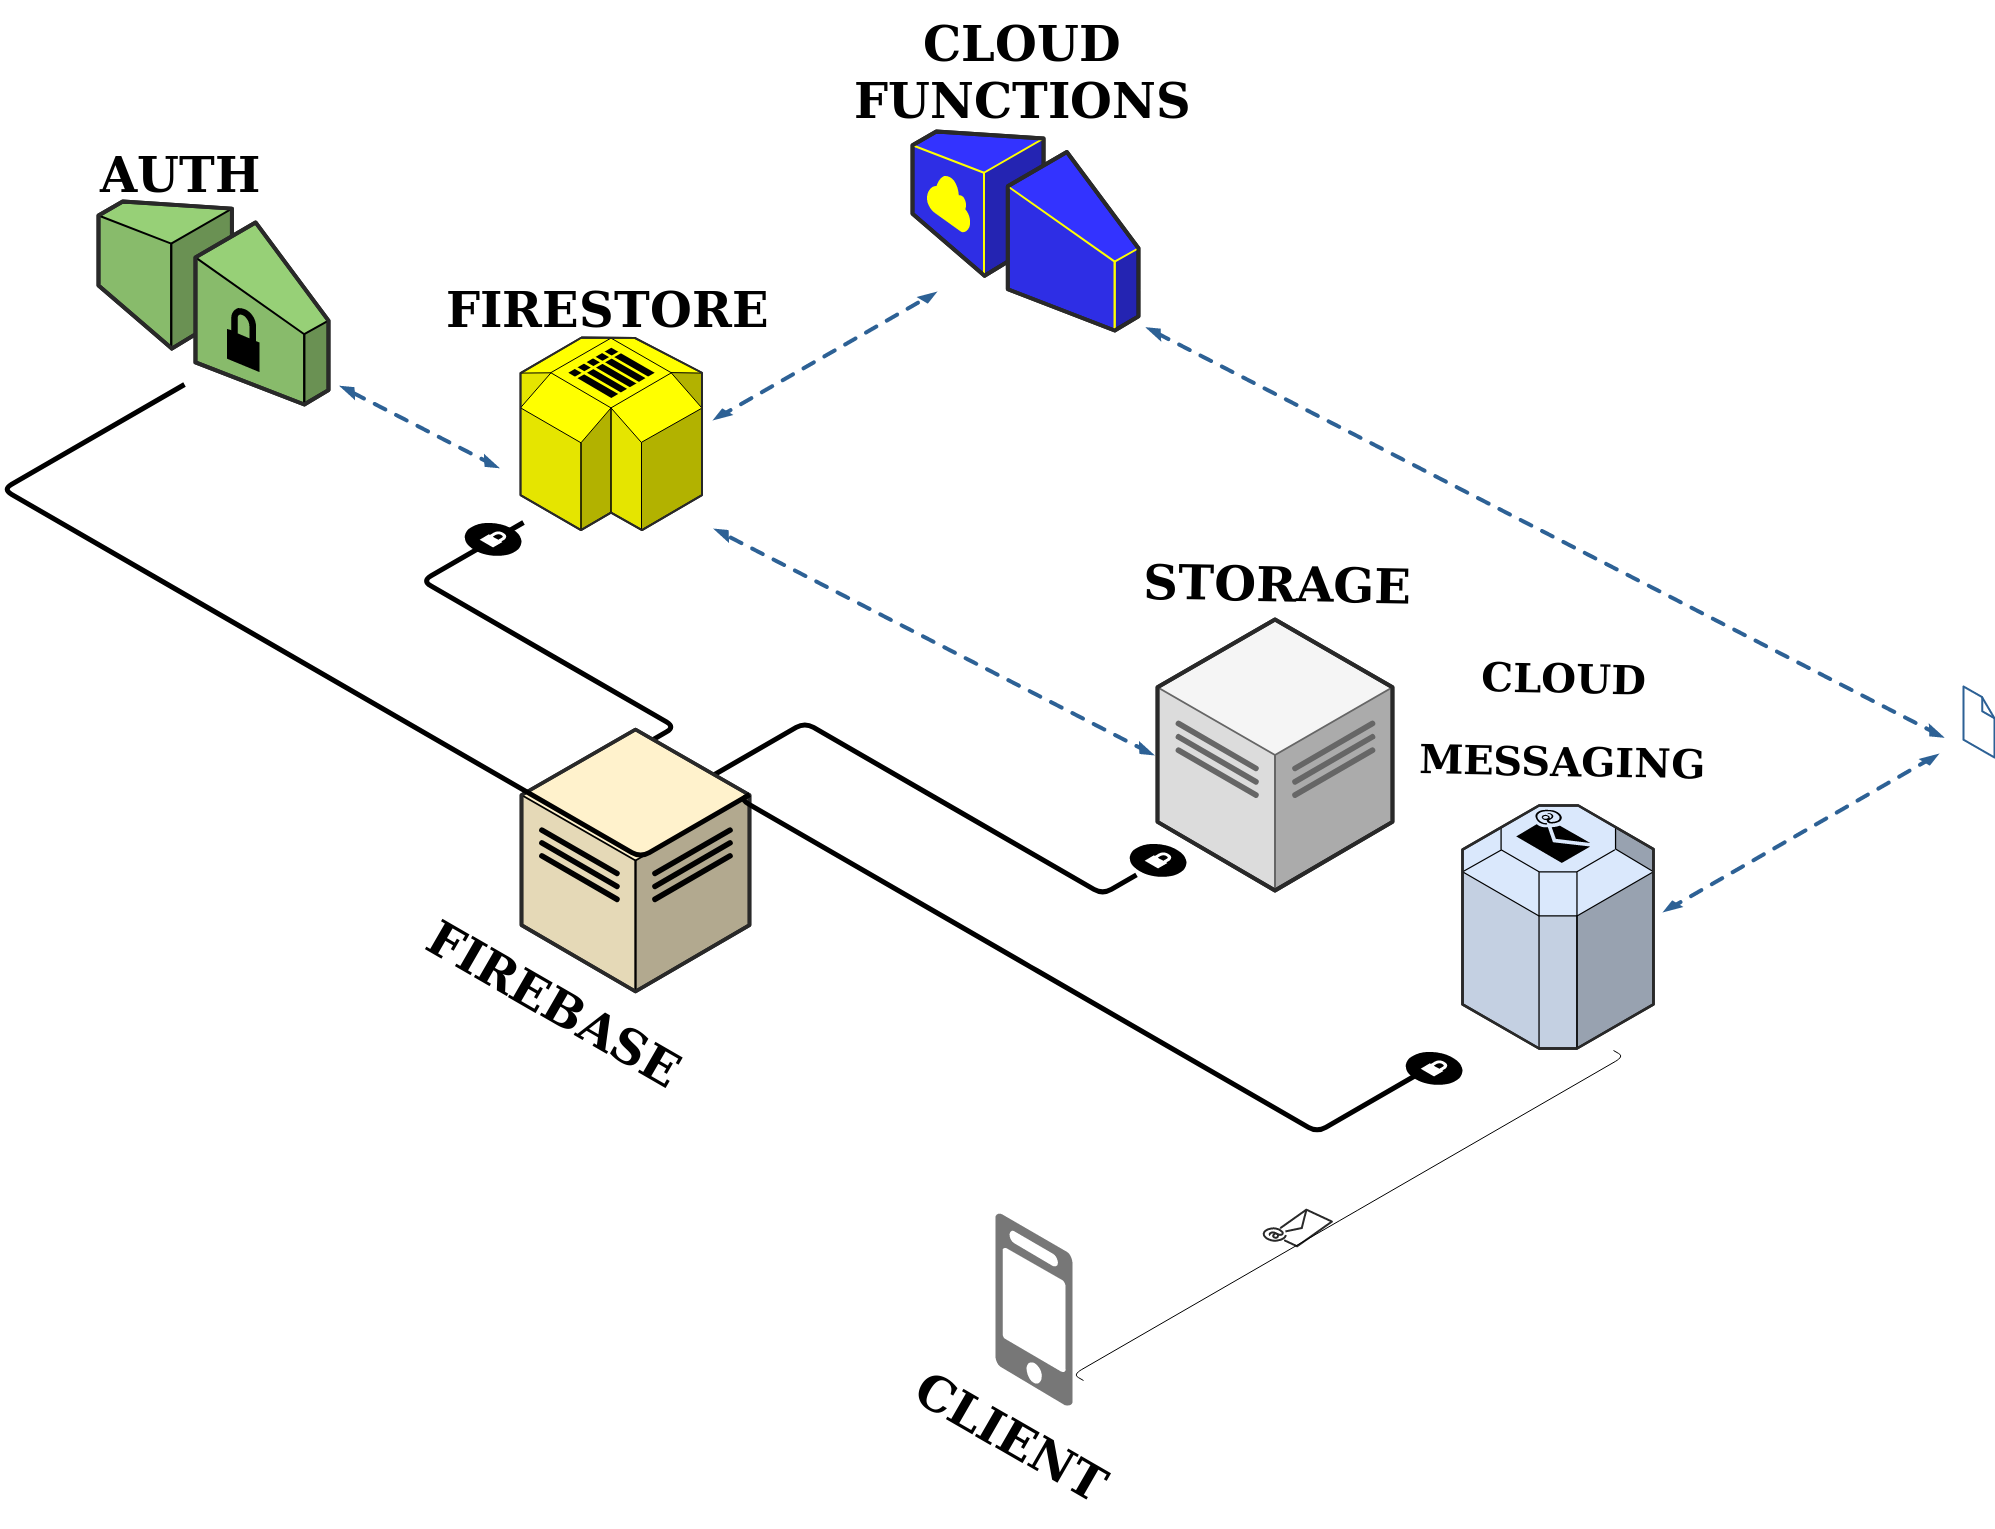
\includegraphics[width=0.7\textwidth]{immagini/server_arch.png}
  \caption{Server Architettura}\label{fig:Architettura Server}
\end{figure}


\section{Model View Presenter}                 %crea la sezione
MVP (Model View Presenter) \'e un pattern architetturale utilizzato per l'organizzazione strutturale di un progetto, in modo da trarne vantaggio in termini di prestazioni, leggibilit\'a e modularit\'a del codice.\\
La sua caratteristica principale \'e quella di separare il livello di presentazione dalla logica, in modo che tutto ci\'o che riguarda l'interazione dell'utente con l'interfaccia sia separato da come vengono rappresentati i dati.\\
Il pattern MVP deriva dal pattern MVC (Model View Controller), che ha 3 concetti base, che lo definiscono:

\begin{enumerate}
\item Model: Il modello dei dati da visualizzare
\item View: L'interfaccia utente che visualizza i dati
\item Controller: Controlla l'interazione tra Model e View
\end{enumerate}

La principale differenza tra i due pattern \'e che il Presenter del MVP gestisce la logica tra la View e il Model, e la sua implementazione permette di gestire l'interfaccia utente ma soprattutto rendere pi\'u comoda l'interazione tra interfaccia utente e i dati.\\


Come il pattern MVC, anche il pattern MVP permette di rendere le View indipendenti dalla gestione dei dati, dividendo la logica dell' applicazione in tre livelli distinti, livelli che possono essere testati separatamente.\\
La possibilit\'a di poter testare i livelli separatamente \'e una delle caratteristiche del MVP.\@


\begin{enumerate}
\item Model: Il modello \'e un' interfaccia che definisce i dati da visualizzare.
\item View: La View \'e un' interfaccia passiva che visualizza i dati (il modello) e instrada i comandi utente (eventi) al Presenter per agire su tali dati.
\item Presenter: Il Presenter agisce sul modello e sulla vista. Recupera i dati dai repository (il modello) e li formatta per la visualizzazione nella vista.
\end{enumerate}

\begin{figure}[!h]
  \centering
  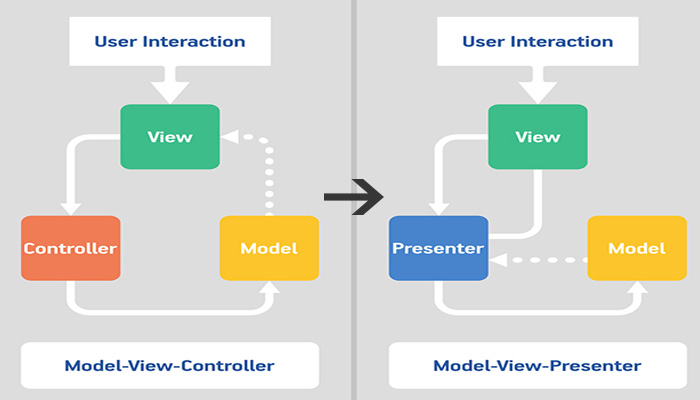
\includegraphics[width=0.65\textwidth]{immagini/mvc-vs-mvp.jpg}
  \caption{MVC vs MVP.}\label{fig:MVC vs MVP}
\end{figure}

\newpage


\subsection{Model}
Il Model \'e un'interfaccia dedicata all'acceso dei dati di un'applicazione, si occupa quindi di fornire un'astrazione del modello dei dati presenti nel database.\\
Il Model oltre a contenere la struttura dei dati da visualizzare si occupa anche di fornire una buona astrazione dei dati presenti nel database, modificando, aggiungendo e separando alcuni dei dati, in modo da rendere l'accesso e la visualizzazione dei dati pi\'u semplice per gli altri due componenti del pattern (View, Presenter).\\
Un esempio potrebbe essere il seguente:
Il database contiene una tabella con due tipi di dato:

\begin{enumerate}
\item \textbf{Nome}: String
\item \textbf{DataDiNascita}: Date
\end{enumerate}

Quando il programma ricever\'a i dati dal database in un qualsiasi formato( Map, Json, Array..) il Model selezionerà i dati in base alla definizione data dal programmatore trasformando il risultato del database in un oggetto.
Questo oggetto oltre a conserare le due informazioni ricevute dal database (Nome, DataDiNascita) potr'\a contenere ance informazioni aggiuntive inserite dal Model per facilitare l'uso e la manipolazione degli altri due componeti.
In questo caso il modello potrebbe creare il nuovo campo "et\'a" facendo una semplice sottrazione fra due date, quella attuale e la data di nascita dell'utente.

\begin{enumerate}
\item \textbf{Nome}: String
\item \textbf{DataDiNascita}: Date
\item \textbf{Et\'a}: Int
\end{enumerate}

%https://medium.com/@cervonefrancesco/model-view-presenter-android-guidelines-94970b430ddf

\subsection{View}
La View \'e un' interfaccia che definisce cosa deve implementare il Presenter, affinch\'e possa interagire con l'interfaccia utente.\\
La View interagisce con il Presenter per visualizzare i dati e notifica al Presenter le azioni che compie l'utente nell'interfaccia.\\
La View pu\'o essere implementata da un Activity, un Fragment, o un widget Android, che contengono ProgressBar, TextView, RecyclerView o altri elementi che necessitano di essere aggiornarnati in base a qualche azione dell'utente o cambiamento nel server.\\
Una delle problematiche riscontrare durante il testing delle view in Android sono causate della complessità del framework.Per risolvere questo problema, attraverso l'utilizzo del pattern MVP è possibile implementare una Passive View( modello di vista passivo).
La sua implementazione riduce al minimo la quantità di logica implementata nella vista.
Ad esempio, se si dispone di un modulo username/password e di un pulsante "Invia", non si scrive la logica di validazione all' interno della View ma all' interno del Presenter. La View infatti dovrebbe solo contenere il nome utente e la password e inviarli al Presenter.



\subsection{Presenter}
Il Presenter \'e il mediatore tra il Model e la View e si occupa di  recuperare i dati dal Model, formattarli e passarli alla View, ma a differenza del pattern MVC, decide anche cosa succede quando si interagisce con la View reagendo alle interazioni dell'utente.\\
Il Presenter per facilitare il testing deve cercare di non dipendere minimamente da Android, ma contenere solo metodi e dipendente Java, senza l'utilizzo del "Context" ad esempio, questo permetter\'a di scrivere i test per il Presenter senza l'utilizzo di un emulatore Android.\\
Come detto in precedenza  il Presenter deve dipendere dall' interfaccia View e non direttamente dall' Activity o Fragment, in questo modo si tengono separati il Presenter e l'Activity rispettando la D dei principi SOLID:"Dipendi dalle astensioni. Non dipendere dalle concrezioni"\\





%%%%%%%%%%%%%%%%%%%%%%%%%%%%%%%%%%%%%%%%%non numera l'ultima pagina sinistra
\clearpage{\pagestyle{empty}\cleardoublepage}
